\documentclass[a4paper, 12pt]{article}

% packages
\usepackage{amssymb}
\usepackage[fleqn]{mathtools}
\usepackage{tikz}
\usepackage{enumerate}
\usepackage{bussproofs}
\usepackage{xcolor}
\usepackage[margin=1.3cm]{geometry}
\usepackage{logicproof}
\usepackage{diagbox}
\usepackage{listings}
\usepackage{graphicx}
\usepackage{lstautogobble}
\usepackage{hyperref}
\usepackage{multirow}
\usepackage{tipa}
\usepackage{pgfplots}
\usepackage{adjustbox}

% tikz libraries
\usetikzlibrary{
    decorations.pathreplacing,
    arrows,
    shapes,
    shapes.gates.logic.US,
    circuits.logic.US,
    calc,
    automata,
    positioning,
    intersections
}

\pgfplotsset{compat=1.16}

\pgfmathdeclarefunction{gauss}{2}{%
  \pgfmathparse{1/(#2*sqrt(2*pi))*exp(-((x-#1)^2)/(2*#2^2))}%
}

\allowdisplaybreaks % allow environments to break
\setlength\parindent{0pt} % no indent

% shorthand for verbatim
% this clashes with logicproof, so maybe fix this at some point?
\catcode`~=\active
\def~#1~{\texttt{#1}}

% code listing
\lstdefinestyle{main}{
    numberstyle=\tiny,
    breaklines=true,
    showspaces=false,
    showstringspaces=false,
    tabsize=2,
    numbers=left,
    basicstyle=\ttfamily,
    columns=fixed,
    fontadjust=true,
    basewidth=0.5em,
    autogobble,
    xleftmargin=3.0ex,
    mathescape=true
}
\newcommand{\dollar}{\mbox{\textdollar}} %
\lstset{style=main}

% augmented matrix
\makeatletter
\renewcommand*\env@matrix[1][*\c@MaxMatrixCols c]{%
\hskip -\arraycolsep
\let\@ifnextchar\new@ifnextchar
\array{#1}}
\makeatother

% ceiling / floor
\DeclarePairedDelimiter{\ceil}{\lceil}{\rceil}
\DeclarePairedDelimiter{\floor}{\lfloor}{\rfloor}

% custom commands
\newcommand{\indefint}[2]{\int #1 \, \mathrm{d}#2}
\newcommand{\defint}[4]{\int_{#1}^{#2} #3 \, \mathrm{d}#4}
\newcommand{\pdif}[2]{\frac{\partial #1}{\partial #2}}
\newcommand{\dif}[2]{\frac{\mathrm{d}#1}{\mathrm{d}#2}}
\newcommand{\limit}[2]{\raisebox{0.5ex}{\scalebox{0.8}{$\displaystyle{\lim_{#1 \to #2}}$}}}
\newcommand{\limitsup}[2]{\raisebox{0.5ex}{\scalebox{0.8}{$\displaystyle{\limsup_{#1 \to #2}}$}}}
\newcommand{\summation}[2]{\sum\limits_{#1}^{#2}}
\newcommand{\product}[2]{\prod\limits_{#1}^{#2}}
\newcommand{\intbracket}[3]{\left[#3\right]_{#1}^{#2}}
\newcommand{\laplace}{\mathcal{L}}
\newcommand{\fourier}{\mathcal{F}}
\newcommand{\mat}[1]{\boldsymbol{#1}}
\renewcommand{\vec}[1]{\boldsymbol{#1}}
\newcommand{\rowt}[1]{\begin{bmatrix}
    #1
\end{bmatrix}^\top}
\DeclareMathOperator*{\argmax}{argmax}
\DeclareMathOperator*{\argmin}{argmin}

\newcommand{\lto}[0]{\leadsto\ }

\newcommand{\ulsmash}[1]{\underline{\smash{#1}}}

\newcommand{\powerset}[0]{\wp}
\renewcommand{\emptyset}[0]{\varnothing}

\makeatletter
\newsavebox{\@brx}
\newcommand{\llangle}[1][]{\savebox{\@brx}{\(\m@th{#1\langle}\)}%
  \mathopen{\copy\@brx\kern-0.5\wd\@brx\usebox{\@brx}}}
\newcommand{\rrangle}[1][]{\savebox{\@brx}{\(\m@th{#1\rangle}\)}%
  \mathclose{\copy\@brx\kern-0.5\wd\@brx\usebox{\@brx}}}
\makeatother
\newcommand{\lla}{\llangle}
\newcommand{\rra}{\rrangle}
\newcommand{\la}{\langle}
\newcommand{\ra}{\rangle}
\newcommand{\crnr}[1]{\text{\textopencorner} #1 \text{\textcorner}}
\newcommand{\bnfsep}[0]{\ |\ }
\newcommand{\concsep}[0]{\ ||\ }

\newcommand{\axiom}[1]{\AxiomC{#1}}
\newcommand{\unary}[1]{\UnaryInfC{#1}}
\newcommand{\binary}[1]{\BinaryInfC{#1}}
\newcommand{\trinary}[1]{\TrinaryInfC{#1}}
\newcommand{\quaternary}[1]{\QuaternaryInfC{#1}}
\newcommand{\quinary}[1]{\QuinaryInfC{#1}}
\newcommand{\dproof}[0]{\DisplayProof}
\newcommand{\llabel}[1]{\LeftLabel{\scriptsize #1}}
\newcommand{\rlabel}[1]{\RightLabel{\scriptsize #1}}

\newcommand{\ttbs}{\char`\\}
\newcommand{\lrbt}[0]{\ \bullet\ }

% colours
\newcommand{\violet}[1]{\textcolor{violet}{#1}}
\newcommand{\blue}[1]{\textcolor{blue}{#1}}
\newcommand{\red}[1]{\textcolor{red}{#1}}
\newcommand{\teal}[1]{\textcolor{teal}{#1}}

% reasoning proofs
\usepackage{ltablex}
\usepackage{environ}
\keepXColumns
\NewEnviron{reasoning}{
    \begin{tabularx}{\textwidth}{rlX}
        \BODY
    \end{tabularx}
}
\newcommand{\proofline}[3]{$(#1)$ & $#2$ & \hfill #3 \smallskip \\}
\newcommand{\proofarbitrary}[1]{& take arbitrary $#1$ \smallskip \\}
\newcommand{\prooftext}[1]{\multicolumn{3}{l}{#1} \smallskip \\}
\newcommand{\proofmath}[3]{$#1$ & = $#2$ & \hfill #3 \smallskip \\}
\newcommand{\prooftherefore}[1]{& $\therefore #1$ \smallskip \\}
\newcommand{\proofbc}[0]{\prooftext{\textbf{Base Case}}}
\newcommand{\proofis}[0]{\prooftext{\textbf{Inductive Step}}}

% ER diagrams
\newcommand{\nattribute}[4]{
    \node[draw, state, inner sep=0cm, minimum size=0.2cm, label=#3:{#4}] (#1) at (#2) {};
}
\newcommand{\mattribute}[4]{
    \node[draw, state, accepting, inner sep=0cm, minimum size=0.2cm, label=#3:{#4}] (#1) at (#2) {};
}
\newcommand{\dattribute}[4]{
    \node[draw, state, dashed, inner sep=0cm, minimum size=0.2cm, label=#3:{#4}] (#1) at (#2) {};
}
\newcommand{\entity}[3]{
    \node[] (#1-c) at (#2) {#3};
    \node[inner sep=0cm] (#1-l) at ($(#1-c) + (-1, 0)$) {};
    \node[inner sep=0cm] (#1-r) at ($(#1-c) + (1, 0)$) {};
    \node[inner sep=0cm] (#1-u) at ($(#1-c) + (0, 0.5)$) {};
    \node[inner sep=0cm] (#1-d) at ($(#1-c) + (0, -0.5)$) {};
    \draw
    ($(#1-c) + (-1, 0.5)$) -- ($(#1-c) + (1, 0.5)$) -- ($(#1-c) + (1, -0.5)$) -- ($(#1-c) + (-1, -0.5)$) -- cycle;
}
\newcommand{\relationship}[3]{
    \node[] (#1-c) at (#2) {#3};
    \node[inner sep=0cm] (#1-l) at ($(#1-c) + (-1, 0)$) {};
    \node[inner sep=0cm] (#1-r) at ($(#1-c) + (1, 0)$) {};
    \node[inner sep=0cm] (#1-u) at ($(#1-c) + (0, 1)$) {};
    \node[inner sep=0cm] (#1-d) at ($(#1-c) + (0, -1)$) {};
    \draw
    ($(#1-c) + (-1, 0)$) -- ($(#1-c) + (0, 1)$) -- ($(#1-c) + (1, 0)$) -- ($(#1-c) + (0, -1)$) -- cycle;
}

% AVL Trees
\newcommand{\avltri}[4]{
    \draw ($(#1)$) -- ($(#1) + #4*(0.5, -1)$) -- ($(#1) + #4*(-0.5, -1)$) -- cycle;
    \node at ($(#1) + #4*(0, -1) + (0, 0.5)$) {#3};
    \node at ($(#1) + #4*(0, -1) + (0, -0.5)$) {#2};
}

% RB Trees
\tikzset{rbtr/.style={inner sep=2pt, circle, draw=black, fill=red}}
\tikzset{rbtb/.style={inner sep=2pt, circle, draw=black, fill=black}}

% Samples
\tikzset{spos/.style={inner sep=2pt, circle, draw=black, fill=blue!20}}
\tikzset{sneg/.style={inner sep=2pt, circle, draw=black, fill=red!20}}

% Joins
\newcommand\ljoin{\stackrel{\mathclap{\normalfont\mbox{\tiny L}}}{\bowtie}}
\newcommand\rjoin{\stackrel{\mathclap{\normalfont\mbox{\tiny R}}}{\bowtie}}
\newcommand\ojoin{\stackrel{\mathclap{\normalfont\mbox{\tiny O}}}{\bowtie}}

\setcounter{MaxMatrixCols}{100}

% actual document
\begin{document}
    {\sc Computing $4^\text{th}$ Year Notes} \hfill ~https://github.com/lin-e/imperial-revision~
    \rule{\textwidth}{0.1pt}
    \section*{Scalable Systems and Data \hfill (70022)}
        \subsection*{1.1 - Database Storage Layer}
            This lecture covers the DBMS layers, storage hierarchy as well as the role disks takes in the DBMS.
            The DBMS layers are as follows, with the query going into the first layer, and storage being the final layer.
            Note that the last two layers (buffer management and disk space management are typically done by the OS).
            \begin{enumerate}[1.]
                \itemsep0em
                \item \textbf{query optimization and execution} \hfill tries to reorganise the query to execute efficiently
                \item \textbf{relational operators}
                \item \textbf{file and access methods} \hfill understand which files need to be accessed and indexes we can use
                \item \textbf{buffer management} \hfill handles reading disk pages and buffering in main memory for fast access
                \item \textbf{disk space management}
            \end{enumerate}
            An example of this could be a search engine, which is much simpler than a general DBMS - albeit having similar layers;
            \begin{enumerate}[1.]
                \itemsep0em
                \item search string modifier
                \item ranking engine
                \item query execution
                \item buffer management
                \item disk space management
            \end{enumerate}
            This is simpler than a DBMS as it can simply use the OS for the bottom two layers, there is typically no concurrency (nor any need for transactions, being mostly read-only), and typically has hard-wired queries.
            The ranking engine and query execution is a simple DBMS.
            \subsubsection*{DBMS versus Using OS}
                An important question is why we don't simply use the OS.
                The layers of abstractions can be useful, but we have a lot of knowledge on how to access the data.
                In addition, the OS can often get in the way of the DBMS - it has some idea on what to query and what files to touch, and knows more about the OS regarding future access, which can be exploited.
                A DBMS needs to do things its own way, for example specialised pre-fetching with the knowledge of future access.
                Additionally, if we control the buffer management, we can also control the replacement policy, likely with something better than the OS.
                With more control over the thread / process scheduling, the DBMS can achieve a more optimal execution of the workflow as the DB locks aren't going to conflict with the OS locks (high contention).
                There's also control over flushing data to the disk, including writing log file (important for recovery), and shouldn't be left to the OS.
            \subsubsection*{Disks and Files}
                Today, disks are still the go-to storage medium for large amounts of files, and have become fairly affordable (not as affordable as tape for archival storage, but much cheaper than other media, such as SSD or main memory).
                Unlike other media, disks have mechanical parts leading to differences access patterns or behaviour - the time to access a piece of data is affected by \textbf{where} the data is on the disk.
                A lot of databases today are still on disks, as it's cheap with a reasonable access time - typically the data is read from the disk onto main memory (buffered), and changes are written back to the disk from the buffer.
                \medskip

                High-end databases are in the petabyte range, therefore using main memory would be extremely expensive.
                In addition to that, main memory is volatile - meaning the data is lost if power goes out.
                However, main-memory databases do exist for smaller sized, performance optimised systems, in which volatility is tolerable.
                \medskip

                Flash storage isn't commonly used in DBMS as main storage (due to the cost), but can also be used as an accelerator or enabler, in the form of a specialised cache, etc.
                \medskip

                The storage hierarchy is as follows.
                Note that flash storage can either be used to the side of magnetic disk (for a specific portion of the files), or as a buffer on top (before main memory).
                \textit{Jim Gray} has an analogy for how far away the data is (registers being knowledge in your head, etc), illustrating the scale of access time.
                \begin{center}
                    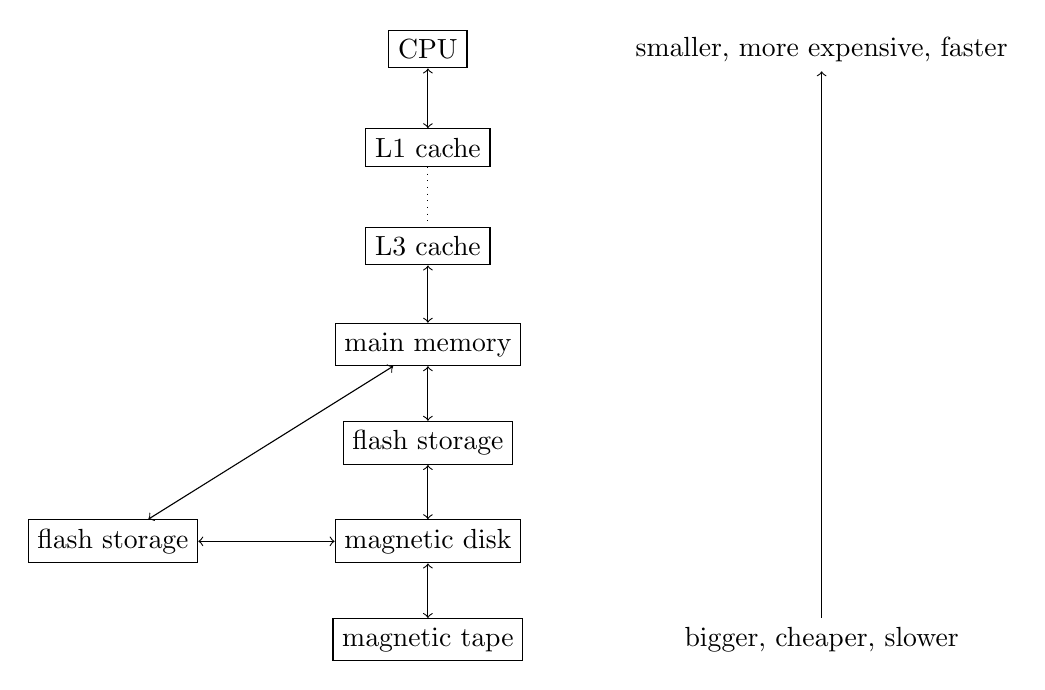
\begin{tikzpicture}[y=1.25cm]
                        \node[draw] (cpu) at (0, 0) {CPU};
                        \node[draw] (l1) at (0, -1) {L1 cache};
                        \node[draw] (l3) at (0, -2) {L3 cache};
                        \node[draw] (mm) at (0, -3) {main memory};
                        \node[draw] (fs1) at (0, -4) {flash storage};
                        \node[draw] (md) at (0, -5) {magnetic disk};
                        \node[draw] (fs2) at (-4, -5) {flash storage};
                        \node[draw] (mt) at (0, -6) {magnetic tape};

                        \draw
                        (cpu) edge[<->] (l1)
                        (l1) edge[dotted] (l3)
                        (l3) edge[<->] (mm)
                        (mm) edge[<->] (fs1)
                        (mm) edge[<->] (fs2)
                        (fs1) edge[<->] (md)
                        (fs2) edge[<->] (md)
                        (md) edge[<->] (mt);

                        \node (x) at (5, -6) {bigger, cheaper, slower};
                        \node (y) at (5, 0) {smaller, more expensive, faster};

                        \draw (x) edge[->] (y);
                    \end{tikzpicture}
                \end{center}
                Disks are still the main secondary storage device of choice, with the main advantage over tapes being the ability to perform random access, rather than purely sequential.
                Data is stored in units in \textbf{disk blocks} or \textbf{pages} (may be used interchangeably), typically in the order of kilobytes and occasionally megabytes.
                Unlike RAM, the time to retrieve / write a disk page varies depending on the location, with a tremendous impact on time to retrieve, hence relative placement of pages on a disk has a major impact on performance.
                The lecture then goes over the anatomy of a disk;
                \begin{itemize}
                    \itemsep0em
                    \item spindle and platters spin between 5,000 - 15,000 RPM (with physical limitations)
                    \item arm assembly has multiple disk head, one for each platter - the tracks under the heads form a cylinder
                    \item only one head reads or writes at once
                \end{itemize}
                The time to access a disk block has three elements;
                \begin{itemize}
                    \itemsep0em
                    \item \textbf{seek time} \hfill time to move the arm to the correct position (in and out, towards the spindle)
                    \item \textbf{rotational delay} \hfill arm assembly in a fixed position, block needs to be rotated under head
                    \item \textbf{transfer time} \hfill actual time to read data from disk into main memory
                \end{itemize}
                The time for a smaller number of cylinders traversed is dominated by the seek time (head positioning).
                In modern disks, short seeks are dominated by the \textbf{settle time}, which gets larger with increased disk track density.
                \medskip

                Generally, the seek time and rotational delay dominates, with the former being in the range of 1 to 20ms, and the latter being in the range of 0 to 10ms.
                On the other hand, the transfer rate is less than 1 millisecond for a 4KB page.
                As such, the key to lower I/O cost is to reduce the delays caused by seek and rotation.
                Additionally, in shared disks, most of the time is spent waiting for access to the arm.
                \medskip

                The concept of the next block is as follows;
                \begin{itemize}
                    \itemsep0em
                    \item blocks on the same track, followed by
                    \item blocks on the same cylinder
                    \item blocks on adjacent cylinder
                \end{itemize}
                We can't control where we write on the disk - that's controlled by the device driver.
                Typically, if data is written together, it will also be read together.
                Defragmentation is disk optimization, as data can be spread out all over a disk for a given file, leading to slower read times - this is done by putting all the pieces of a file closer together.
                \medskip

                Note that an adjacent block doesn't necessarily mean physically adjacent.
                Data can be physically spread out over a disk but in a certain pattern that can lead to near sequential access.
                The adjacent blocks can be the blocks under the disk head after rotating during settle time.
                \medskip

                In general, memory access is much faster than disk I/O (roughly $1,000 \times$), and sequential I/O is faster than random (roughly $10 \times$).
                \medskip

                The lowest layer of DBMS manages the space on the disk and higher levels can call this layer to allocate / de-allocate a page, or read / write a page.
            \subsubsection*{Summary}
                In general, the key for storing data on a disk is to store data together if it's queried together.
                Random access should be avoided, preferably use sequential access.
                Data structures should be aligned for page size - for example, if a data structure were to have a few bytes in the next page, an additional page would have to be retrieved, despite mostly being irrelevant.
        \subsection*{1.2 - Main Memory Indexing}
            The general trend is that we have more main memory as time goes on.
            The hardware trends show that CPU speed and main memory capacity doubles every 18 months, however memory speed only grows by 10\% per year.
            \medskip

            This means that many databases, typically OLTP, can fit into main memory; OLAP is still in the order of petabytes, if not more.
            Memory access has become the new bottleneck for main memory databases.
            There is no longer a uniform random access model (NUMA), meaning that we can no longer assume that accessing each piece of data in memory takes the same amount of time.
            Cache performance has become crucial.
            \medskip

            The memory hierarchy is as follows.
            Note that a cache \textbf{line} is the smallest unit that can be retrieved from the cache, and data structures should be aligned to a line in a similar way to pages.
            \begin{itemize}
                \itemsep0em
                \item CPU (registers)
                \item L1 cache, takes 1 cycle, 8-64 KB, 32 bytes per line
                \item L2 cache, takes 2 - 10 cycles, 64 - 128 bytes per line
                \item TLB, takes 10 - 100 cycles, 64 entries / pages
            \end{itemize}
            The cache performance is crucial, similar to the disk cache / buffer pool, however the DBMS doesn't have direct control of this.
            \subsubsection*{Improving Cache Performance}
                The primary factors are the cache capacity and data locality, the former is a given and can't be changed, whereas we can do something about the locality.
                An example with non-random access, such as a scan or index traversal is by clustering data structures to a multiple of a cache line, as well as squeezing more useful data into a cache line.
                On the other hand, with random access, such as in a hash join, the data should be partitioned to fit in cache / TLB.
                CPU is often also traded for memory access, such as compression (requires more CPU processing, but reduces storage usage).
            \subsubsection*{Trees}
                The lecture then goes through an example of a tree index, where each node holds 2 entries.
                Each node can point to three other nodes, where the values are either below, in between the two values, or higher than both.
                \medskip

                The B+ tree is quite similar, but all leaf nodes are connected.
                This allows for faster execution of range queries, as the nodes are connected without traversing up and down the tree.
                The \textbf{order} is the minimum number of keys or pointers in a non-leaf node and the \textbf{fanout} of a node is the number of pointers out of the node.
                These have the following properties;
                \begin{itemize}
                    \itemsep0em
                    \item balanced - leaves are at the same level, leading to predictable performance when traversing down the tree (same for every node)
                    \item every node, other than the root, must be at least half full meaning it becomes balanced
                    \item searching is $\log_d(n)$, where $d$ is the order and $n$ is the number of entries
                    \item insertion involves finding the leaf to insert to, splitting if the node is full and adjusting index accordingly; has a similar cost to searching, have to find all the way down, and may have to split all the way back up
                    \item deletion is similar, find leaf node, delete, and merge neighbouring nodes if required (not half-full)
                \end{itemize}
                \textbf{Cache sensitive search trees} can be thought of as a B+ tree that has been optimised specifically for main memory.
                The basic approach for this is to improve locality, with each node of the tree fitting into an L2 cache line, as the penalty of an L2 miss is significantly higher than that of an L1 miss, and can fit more nodes in L2 than L1.
                Keys are fixed length (from variable length) by the use of dictionary compression, letting us know the size of a child node.
                Child pointers are also eliminated; previously we had multiple pointers to point to each of the child nodes, however we now only need one pointer to a single child node as we know the size.
                \begin{center}
                    \begin{tikzpicture}
                        \begin{scope}[shift={(0, 0)}]
                            \begin{scope}[shift={(0, 0)}]
                                \node at (0, 0) {$2$};
                                \draw
                                (-1, -0.5) -- (1, -0.5) -- (1, 0.5) -- (-1, 0.5) -- cycle
                                (-0.5, -0.5) -- (-0.5, 0.5)
                                (0.5, -0.5) -- (0.5, 0.5);
                            \end{scope}
                            \begin{scope}[shift={(-1.5, -2)}]
                                \node at (0, 0) {$1$};
                                \draw
                                (-1, -0.5) -- (1, -0.5) -- (1, 0.5) -- (-1, 0.5) -- cycle
                                (-0.5, -0.5) -- (-0.5, 0.5)
                                (0.5, -0.5) -- (0.5, 0.5);
                            \end{scope}
                            \begin{scope}[shift={(1.5, -2)}]
                                \node at (0, 0) {$3$};
                                \draw
                                (-1, -0.5) -- (1, -0.5) -- (1, 0.5) -- (-1, 0.5) -- cycle
                                (-0.5, -0.5) -- (-0.5, 0.5)
                                (0.5, -0.5) -- (0.5, 0.5);
                            \end{scope}
                            \begin{scope}[shift={(-3, -4)}]
                                \node at (0, 0) {$1$};
                                \draw
                                (-0.5, -0.5) -- (1, -0.5) -- (1, 0.5) -- (-0.5, 0.5) -- cycle
                                (0.5, -0.5) -- (0.5, 0.5);
                            \end{scope}
                            \begin{scope}[shift={(-1, -4)}]
                                \node at (0, 0) {$2$};
                                \draw
                                (-0.5, -0.5) -- (1, -0.5) -- (1, 0.5) -- (-0.5, 0.5) -- cycle
                                (0.5, -0.5) -- (0.5, 0.5);
                            \end{scope}
                            \begin{scope}[shift={(1, -4)}]
                                \node at (0, 0) {$3$};
                                \draw
                                (-0.5, -0.5) -- (1, -0.5) -- (1, 0.5) -- (-0.5, 0.5) -- cycle
                                (0.5, -0.5) -- (0.5, 0.5);
                            \end{scope}
                            \begin{scope}[shift={(3, -4)}]
                                \node at (0, 0) {$4$};
                                \draw
                                (-0.5, -0.5) -- (1, -0.5) -- (1, 0.5) -- (-0.5, 0.5) -- cycle
                                (0.5, -0.5) -- (0.5, 0.5);
                            \end{scope}

                            \draw
                            (-0.75, 0) edge[->] (-1.5, -1.5)
                            (0.75, 0) edge[->] (1.5, -1.5)
                            (-2.25, -2) edge[->] (-3, -3.5)
                            (-0.75, -2) edge[->] (-1, -3.5)
                            (0.75, -2) edge[->] (1, -3.5)
                            (2.25, -2) edge[->] (3, -3.5)
                            (-2.25, -4) edge[->] (-2.25, -5)
                            (-0.25, -4) edge[->] (-0.25, -5)
                            (1.75, -4) edge[->] (1.75, -5)
                            (3.75, -4) edge[->] (3.75, -5);
                        \end{scope}

                        \begin{scope}[shift=({10, 0})]
                            \draw
                            (-1.5, 0.5) -- (1.5, 0.5) -- (1.5, -0.5) -- (-1.5, -0.5) -- cycle
                            (-0.5, 0.5) -- (-0.5, -0.5)
                            (0.5, 0.5) -- (0.5, -0.5);
                            \node at (-1, 0) {$1$};
                            \node at (0, 0) {$2$};
                            \node at (1, 0) {$3$};

                            \begin{scope}[shift={(-3, -4)}]
                                \node at (0, 0) {$1$};
                                \draw
                                (-0.5, -0.5) -- (1, -0.5) -- (1, 0.5) -- (-0.5, 0.5) -- cycle
                                (0.5, -0.5) -- (0.5, 0.5);
                            \end{scope}
                            \begin{scope}[shift={(-1, -4)}]
                                \node at (0, 0) {$2$};
                                \draw
                                (-0.5, -0.5) -- (1, -0.5) -- (1, 0.5) -- (-0.5, 0.5) -- cycle
                                (0.5, -0.5) -- (0.5, 0.5);
                            \end{scope}
                            \begin{scope}[shift={(1, -4)}]
                                \node at (0, 0) {$3$};
                                \draw
                                (-0.5, -0.5) -- (1, -0.5) -- (1, 0.5) -- (-0.5, 0.5) -- cycle
                                (0.5, -0.5) -- (0.5, 0.5);
                            \end{scope}
                            \begin{scope}[shift={(3, -4)}]
                                \node at (0, 0) {$4$};
                                \draw
                                (-0.5, -0.5) -- (1, -0.5) -- (1, 0.5) -- (-0.5, 0.5) -- cycle
                                (0.5, -0.5) -- (0.5, 0.5);
                            \end{scope}

                            \draw
                            (-1.5, -0.5) edge[dotted, ->] (-3, -3.5)
                            (-0.5, -0.5) edge[dotted, ->] (-1, -3.5)
                            (0.5, -0.5) edge[dotted, ->] (1, -3.5)
                            (1.5, -0.5) edge[dotted, ->] (3, -3.5)
                            (-2.25, -4) edge[->] (-2.25, -5)
                            (-0.25, -4) edge[->] (-0.25, -5)
                            (1.75, -4) edge[->] (1.75, -5)
                            (3.75, -4) edge[->] (3.75, -5);
                        \end{scope}
                    \end{tikzpicture}
                \end{center}
                In the example above, we assume a cache line size of 24 bytes, a key size (and pointer size) of 4 bytes.
                The B+ tree on the left is 2-way, with 3 misses, and the CSS tree is 4-way, with only 2 misses.
                \medskip

                CSS has the best search / space balance; second best search to hash, which has poor space, and also second best space to binary search, which has poor search.
                The space taken is roughly half that of a B+ tree.
                However, this cannot support dynamic updates as the fan-out and array size must both be fixed.
                \medskip

                A \textbf{CSB+} tree addresses this.
                Children of the same node are stored in an array / node group and the parent only has a single pointer to the child array.
                This has a similar search performance to the CSS tree, and has good update performance if no split occurs.
                Splits are still required as we still have a maximum capacity of an array, which requires allocating new memory.
                \medskip

                A variant of this is a CSB+ tree with segments; the child array is divided into segments, typically 2, with one child pointer per segment.
                This improves split performance, but worsens search performance.
                Another variant is a full CSB+ tree, which is a CSB+ tree with a pre-allocated children array, obviously requiring more space but is good for search and insertion (no more memory needs to be allocated, as it's all allocated).
                It's important to note that none of these are as \textbf{flexible} as B+ trees, but perfectly fine for certain workloads.
                \medskip

                The general performance is as follows, for search, CSS is fastest, followed by full CSB+ (joined with CSB+), then followed by CSB+ with segments, and finally B+.
                On the other hand, with insertion, B+ has the best, roughly equal to full CSB+, which is followed by CSB+ with segments, then CSB+, and finally CSS.
                Generally, full CSB+ is ideal if space isn't a concern, CSB+ (and with segments) is ideal if there are more reads than insertions, and finally CSS is best when read-only.
            \subsubsection*{Cache Conscious Join Method}
                Typically, in vertical decomposed storage, what we want to do when we join in main memory is to partition a base table into $m$ arrays, where $m$ is the number of attributes.
                Variable length fields should also be converted to fixed length fields via the use of dictionary compression.
                For example;
                \begin{center}
                    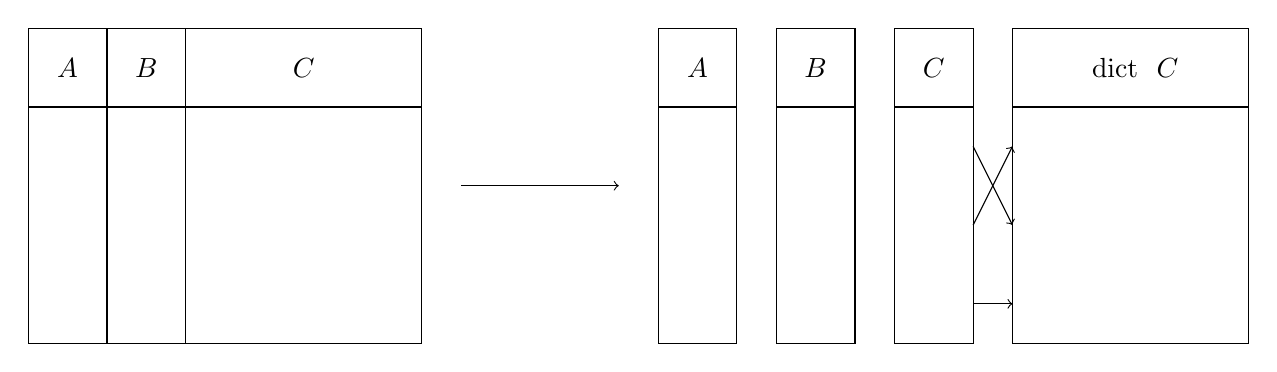
\begin{tikzpicture}[x=0.5cm]
                        \draw
                        (0, 0) -- (10, 0) -- (10, -4) -- (0, -4) -- cycle
                        (0, -1) -- (10, -1)
                        (2, 0) -- (2, -4)
                        (4, 0) -- (4, -4);
                        \node at (1, -0.5) {$A$};
                        \node at (3, -0.5) {$B$};
                        \node at (7, -0.5) {$C$};

                        \draw (11, -2) edge[->] (15, -2);
                        \draw
                        (16, 0) -- (18, 0) -- (18, -4) -- (16, -4) -- cycle
                        (16, -1) -- (18, -1)
                        (19, 0) -- (21, 0) -- (21, -4) -- (19, -4) -- cycle
                        (19, -1) -- (21, -1)
                        (22, 0) -- (24, 0) -- (24, -4) -- (22, -4) -- cycle
                        (22, -1) -- (24, -1)
                        (25, 0) -- (31, 0) -- (31, -4) -- (25, -4) -- cycle
                        (25, -1) -- (31, -1)
                        (24, -1.5) edge[->] (25, -2.5)
                        (24, -2.5) edge[->] (25, -1.5)
                        (24, -3.5) edge[->] (25, -3.5);
                        \node at (17, -0.5) {$A$};
                        \node at (20, -0.5) {$B$};
                        \node at (23, -0.5) {$C$};
                        \node at (28, -0.5) {~dict~ $C$};
                    \end{tikzpicture}
                \end{center}
                Each array contains a pair of OID (uniquely identifies an entry) and value for the $i^\text{th}$ attribute.
                Reconstruction is a simple array access in this case.
                Joins are much more efficient, as we no longer have to read all the data.
                \medskip

                The existing equal-join methods;
                \begin{itemize}
                    \itemsep0em
                    \item sort-merge
                        \subitem one of the relations will not fit in cache, likely meaning we have to read into cache multiple times (take smaller of two relations in main memory)
                    \item hash join \hfill bad if the inner relation doesn't fit into cache
                    \item clustered hash join
                        \subitem one pass to generate cache-sized partitions, take each partition and join it with the other relation, and so on, best of the three solutions, but can be bad if the number of partitions exceed the number of cache lines / TLB entries - can lead to cache thrashing
                \end{itemize}
                This can be addressed with \textbf{radix join}, which first partitions one of the relations and ensure that we partition it into partitions such that we have matching partitions based on $B$ bits of the attribute.
                Matching partitions are joined, nested-loop can be done for small ($\leq 8$ tuples) partitions or a hash join for larger partitions, which is $\leq$ L1 cache, L2 cache, or TLB size (with L1 being ideal).
                This avoids thrashing, compared to clustered hash join.
                Saving these cache misses outweighs the cost of performing extra partitions.
            \subsubsection*{Conclusion}
                The cache performance is important and will become more important as main memory grows.
                The key to this is to cluster data (into a cache line); data that is read together should be written and stored together.
                Irrelevant data should be omitted, including pointers and the use of vertical decomposition.
                Partitions should be done to avoid thrashing.
            \subsubsection*{Spatial Data}
                Spatial data is data with any three dimensions; such as points.
                It has queries such as range queries, nearest neighbours, etc.
                Objects near each other should be stored on the same disk page / cache line, however, there isn't an ordering on data in three dimensions (two objects that are close in 1 dimension could be far apart in another).
                \medskip

                This then goes over an example with reducing computation.
                In the example, checking a range on non-uniform (spatial) partitioning is expensive, as there are many irrelevant points.
                The computation is reduced by using several grids of varying detail; if the range covers the majority of a cell it's checked on that level of detail, if not, it's checked on a lower level of detail.
        \subsection*{October 14 - Live Lecture}
            Learned indexing combines machine learning with indexing.
            The same concept of an index applies, but machine learning models aid to accelerate this lookup, for example by learning distributions.
            These models are typically small and simple, such as interpolation - however, they understand distributions better than existing structures such as B trees.
            The primary challenge is that these models need to fit into main memory, or even the cache to be faster.
            \medskip

            The fundamental problem of a join is to join two relations on a shared attribute.
            If one of the iterations is small, you can iterate over the smaller relation and lookup the related element in the larger relation.
            There are typically two phases in a join, with a build (scanning through the smaller relation and building a hash table), and a probe phase where the second input relation is scanned, and the hash table of the first relation is probed for the matching tuple.
            The problem with this is when the hash table is large, leading to a large number of cache misses.
            One solution is to ensure the hash table can be broken into chunks that fit into cache.
            However, if there are too many partitions, the build phase involves many writes into different partitions, leading to many writes into different locations (thus leading to many TLB misses).
            The radix join addresses this by iteratively partitioning into cache. % ?
            \medskip

            The data in a B+ tree exists in the leaves.
            Any other numbers in internal nodes only exist to help guide the search.
            \medskip

            An adjacent block doesn't necessarily mean a short / small seek distance.
            The abstract concept of an adjacent block could also be called a temporally close block; could be short seek distance or based on rotation.
            Note that the platter is rotating constantly, and by the time the head has finished moving, a different block would be under the head, not necessarily one that is physically nearby.
            If data is written together, it will be stored on adjacent (the abstract concept) blocks, which may still be spread over the disk physically.
            \medskip

            When there's indexing in main memory, the performance is so much faster, the index needs much fewer instructions, otherwise it may be faster to just scan.
            On the other hand, on disks, the performance is relatively slower, allowing for more complex indices.
            This applies even for high-throughput devices.
            \medskip

            DBMS doesn't typically bypass the OS, at least not without a custom OS or specific hardware.
            However, it organises its files or data separately, not leaving it to the OS, as well as handling its own cache and database pages (managed by the database system itself).
            Typically, database systems stores the data in and builds on the OS filesystem.
            You can't force the disk to read / write in a specific physical location, but you can help it write in one go.
\end{document}